\documentclass[journal]{IEEEtran}
\usepackage{amsmath,amssymb}
\usepackage{booktabs,array,graphicx}
\usepackage[ruled,vlined,linesnumbered,noend]{algorithm2e}
\usepackage[hidelinks]{hyperref}
\SetAlgoSkip{}\SetAlgoInsideSkip{}
\hyphenation{sched-ext tail-latency}
\newcommand{\MAINTAB}{%
Bursty mixed & EEVDF & 4.31 & 31.04 & 72.2 [66.5, 78.1] & 56.6 & 1.80 & 8.88 & 54 \\
 & Static FaaS Prio. & 1.73 & 13.16 & 18.8 [16.3, 22.4] & 26.6 & 1.82 & 9.92 & 211 \\
 & LAVD-like & 1.21 & 27.08 & 64.6 [58.3, 70.2] & 22.6 & 1.81 & 9.08 & 109 \\
 & IA-SchedExt & 2.27 & 14.30 & 20.2 [18.0, 23.7] & 36.1 & 1.83 & 10.03 & 205 \\
\midrule
Smooth mixed & EEVDF & 2.66 & 12.90 & 25.8 [24.9, 26.7] & 41.3 & 1.75 & 3.29 & 11 \\
 & Static FaaS Prio. & 1.07 & 4.86 & 9.3 [9.0, 9.5] & 1.6 & 1.77 & 3.37 & 23 \\
 & LAVD-like & 1.03 & 10.96 & 23.4 [22.7, 24.4] & 16.9 & 1.76 & 3.26 & 13 \\
 & IA-SchedExt & 1.47 & 7.45 & 14.3 [14.0, 14.5] & 12.6 & 1.78 & 3.28 & 17 \\
}
\newcommand{\PAIREDTAB}{%
Bursty & vs.\ EEVDF & -71.5\% & [-72.9, -71.0] & $5.3\times10^{-15}$ \\
Bursty & vs.\ LAVD-like & -68.3\% & [-69.2, -67.2] & $5.3\times10^{-15}$ \\
Bursty & vs.\ Static FaaS Prio. & +8.6\% & [+7.3, +9.8] & $5.3\times10^{-15}$ \\
\midrule
Smooth & vs.\ EEVDF & -44.4\% & [-45.3, -43.4] & $5.3\times10^{-15}$ \\
Smooth & vs.\ LAVD-like & -39.0\% & [-40.4, -38.1] & $5.3\times10^{-15}$ \\
Smooth & vs.\ Static FaaS Prio. & +54.9\% & [+52.9, +56.8] & $5.3\times10^{-15}$ \\
}
\newcommand{\SINGLETAB}{%
A (FaaS only) & EEVDF & 0.89 & 8.91 & 0.6 & -- \\
 & Static FaaS Prio. & 0.91 & 8.31 & 1.0 & -- \\
 & LAVD-like & 0.87 & 8.99 & 0.9 & -- \\
 & IA-SchedExt & 0.89 & 8.90 & 0.6 & -- \\
\midrule
B (daemons only) & EEVDF & -- & -- & -- & 3.84 \\
 & Static FaaS Prio. & -- & -- & -- & 3.84 \\
 & LAVD-like & -- & -- & -- & 3.84 \\
 & IA-SchedExt & -- & -- & -- & 3.84 \\
}
\newcommand{\ABLTAB}{%
IA (full) & 20.5 & 36.4 & 207 & 397 \\
no AGING (FAIR/STRICT) & 19.2 & 29.2 & 217 & 389 \\
no STRICT (FAIR/AGING) & 73.4 & 43.5 & 16 & 305 \\
no FAIR (STRICT/AGING) & 20.5 & 36.0 & 208 & 59 \\
theta=0.01 & 20.3 & 36.2 & 207 & 409 \\
theta=0.20 & 22.0 & 38.1 & 209 & 348 \\
F thresholds 0.2/0.5 & 20.3 & 32.9 & 209 & 308 \\
F thresholds 0.4/0.7 & 21.2 & 41.7 & 204 & 407 \\
min dwell 5 ms & 20.3 & 38.1 & 210 & 134 \\
misclassification 5\% & 32.8 & 41.6 & 104 & 460 \\
misclassification 20\% & 58.1 & 49.4 & 47 & 499 \\
}
\newcommand{\GAMMATAB}{%
0.0 & 67.0 & 19.3 & 20.8 \\
0.15 & 69.3 & 19.5 & 20.8 \\
0.3 & 73.0 & 19.7 & 21.1 \\
0.6 & 81.4 & 20.1 & 21.0 \\
}


\begin{document}
\title{Interference-Aware eBPF Scheduling for Mixed Serverless Workloads: A Simulation Study of a Rule-Based \texttt{sched\_ext} Policy}
\author{Mohnish~Tulsian, Chirag~H, and Varshitha~R\\
\IEEEauthorblockA{Department of Computer Science and Engineering (Artificial Intelligence \& Machine Learning)}}
\markboth{IEEE Transactions on Parallel and Distributed Systems}{Tulsian \MakeLowercase{\textit{et al.}}: Interference-Aware eBPF Scheduling for Mixed Serverless Workloads}
\maketitle

\begin{abstract}
Linux EEVDF treats short serverless (FaaS) invocations and long-running background daemons alike, so co-located daemons inflate FaaS tail latency. We specify IA-SchedExt, a deterministic three-mode policy for Linux \texttt{sched\_ext} that switches between fair, strict-priority, and aging dispatch from the FaaS share of runnable tasks and a windowed SLO-miss rate, and evaluate it in an open-source discrete-event simulator against EEVDF, a static FaaS-priority scheduler, and a LAVD-inspired scheduler over 50 paired runs per configuration. On a bursty mixed workload, IA-SchedExt lowers median p99 FaaS latency from 72.2\,ms (EEVDF) to 20.2\,ms ($-71.5\%$, 95\% CI $[-72.9,-71.0]$), and from 64.6\,ms for the LAVD-like baseline ($-68.3\%$), while background throughput is unchanged (1.83 vs.\ 1.80 cores). However, static FaaS priority reaches a lower p99 (18.8\,ms) with no measurable background-throughput cost in any tested regime, so IA-SchedExt is not Pareto-superior to it here. Ablations show that the strict mode accounts for the entire gain and the aging mode adds none, that 5\% task misclassification raises p99 by 60\%, and that the specified mode rule flips modes about 400 times per second. All results are simulation-based; kernel validation is future work.
\end{abstract}

\begin{IEEEkeywords}
Kernel CPU scheduling, eBPF, \texttt{sched\_ext}, serverless, multi-tenant interference, tail latency, EEVDF.
\end{IEEEkeywords}

\section{Introduction}
\IEEEPARstart{F}{unction-as-a-Service} (FaaS) invocations are short (50\,\textmu s--12\,ms), arrive in bursty streams, and carry tight tail-latency SLOs. Linux CFS and its successor EEVDF allocate CPU time without workload classification, so co-located monitoring agents, container runtimes, and analytics daemons cause (i) runqueue head-of-line blocking, (ii) last-level-cache (LLC) eviction, and (iii) memory-bandwidth contention.

The \texttt{sched\_ext} framework (Linux 6.12+) lets eBPF schedulers be loaded at runtime without recompiling the kernel~\cite{schedext}. Existing \texttt{sched\_ext} FaaS schedulers~\cite{metis,emfs} assume FaaS-only hosts. This paper asks whether a simple deterministic, interference-aware policy closes that gap. Contributions: (1) a queueing and LLC interference model; (2) a taxonomy of five open gaps; (3) IA-SchedExt, a three-mode rule-based policy with cgroup-based classification; and (4) an open simulator and a paired evaluation that includes ablations, misclassification and interference-strength sensitivity, and the policy's \emph{negative} results relative to a static-priority baseline.

\section{Background and Problem Formulation}
\subsection{eBPF and \texttt{sched\_ext}}
\texttt{sched\_ext} exposes hooks (\texttt{ops.enqueue}, \texttt{ops.dispatch}, \texttt{ops.select\_cpu}) that eBPF programs override to implement a complete scheduling policy, with automatic fallback on failure~\cite{schedext}. EEVDF runs the eligible task with the earliest virtual deadline
\begin{equation}
d_i=V_i(t)+\frac{q_i}{w_i},
\end{equation}
with slice $q_i$ and weight $w_i$, in $O(\log n)$ time, but is blind to workload class.

\subsection{Cross-Workload Interference Model}
With $T=T_{\mathrm{faas}}\cup T_{\mathrm{bg}}$ and $|T_{\mathrm{bg}}|\gg|T_{\mathrm{faas}}|$, the expected FaaS queueing delay on $C$ cores grows with the service demand $q_j$ queued ahead:
\begin{equation}
\mathbb E[W_{\mathrm{faas}}]=\sum_{j\in Q}\frac{q_j}{C}.
\end{equation}
Background threads also evict FaaS working sets from the LLC, adding a per-access penalty
\begin{equation}
W_{\mathrm{cache}}\approx\frac{S_{\mathrm{bg}}}{L_{\mathrm{LLC}}}\,\big(m_p\,\rho_{\mathrm{miss}}\big),
\end{equation}
where $S_{\mathrm{bg}}$ is the aggregate background working set, $L_{\mathrm{LLC}}$ the LLC capacity, $\rho_{\mathrm{miss}}$ the LLC miss rate, and $m_p\approx150$--$300$\,ns the miss penalty. The simulator realises (2) directly and (3) through two parameters (Section~\ref{sec:eval}).

\section{Research Gaps and Related Work}
\textbf{G1}: eBPF FaaS schedulers~\cite{metis,emfs} do not handle co-scheduled background processes. \textbf{G2}: in-kernel ML inference incurs verifier-bounded overhead~\cite{emfs}. \textbf{G3}: \texttt{sched\_ext} evaluations use isolated FaaS traces~\cite{apsys}. \textbf{G4}: the cost of dynamic scheduler-state switching is unreported. \textbf{G5}: no eBPF scheduler adapts thresholds by feedback control. This paper addresses G1 (in simulation), quantifies mode-switch \emph{rates} and a modelled cost for G4, and measures threshold \emph{sensitivity} for G5 without adapting thresholds; G2 and G3 are out of scope.

Table~\ref{tab:rel} lists the closest work. LAVD~\cite{lavd} is the strongest latency-oriented \texttt{sched\_ext} baseline; control-plane balancing~\cite{platbal} acts at timescales that cannot resolve sub-millisecond contention.

\begin{table}[t]
\centering\footnotesize
\caption{Closest related work.}\label{tab:rel}
\begin{tabular}{@{}p{0.17\columnwidth}p{0.36\columnwidth}p{0.38\columnwidth}@{}}
\toprule
Work & Approach & Limitation\\\midrule
Metis~\cite{metis} & eBPF workflow-aware FaaS scheduler & Serverless-only\\
eMFS~\cite{emfs} & Meta-learning MLFQ CPU predictor & Verifier overhead; no co-daemons\\
APSys~\cite{apsys} & Benchmark of 11 \texttt{sched\_ext} policies & Isolated FaaS only\\
LAVD~\cite{lavd} & Latency-aware \texttt{sched\_ext} for cloud & Not FaaS-burst aware\\
Plat.\ Bal.~\cite{platbal} & Control-plane CPU allocation & Misses sub-ms contention\\
MUSched~\cite{musched} & Interaction-aware mobile scheduler & Mobile domain\\
\bottomrule
\end{tabular}
\end{table}

\section{IA-SchedExt Design}
\subsection{Telemetry and Classification}
On each enqueue, IA-SchedExt reads the FaaS share of runnable tasks $F=N_{\mathrm{faas}}/(N_{\mathrm{faas}}+N_{\mathrm{bg}})$, and the SLO violation rate $R_{\mathrm{miss}}$ over a 100\,ms window (completed invocations plus queued invocations already past the SLO). Tasks are classified as FaaS by cgroup membership (execution-lifetime and CPU-affinity heuristics are specified but not simulated), cached in a TGID-keyed hash map for $O(1)$ lookup.

\subsection{Three-Mode Dispatch}
\begin{equation}
\text{mode}=\begin{cases}
\text{STRICT}, & F>0.60\ \wedge\ R_{\mathrm{miss}}>\theta_{\mathrm{slo}},\\
\text{FAIR}, & F<0.30,\\
\text{AGING}, & \text{otherwise},
\end{cases}
\end{equation}
with $\theta_{\mathrm{slo}}=0.05$. \textbf{FAIR} is EEVDF. \textbf{STRICT} dispatches FaaS tasks first and lets them preempt running background tasks immediately. \textbf{AGING} boosts FaaS tasks by giving them deadline $V+q/B$ and ages background tasks, $V^{\mathrm{aged}}_{\mathrm{bg}}=V_{\mathrm{bg}}-\alpha\,\Delta t$ ($\Delta t$ = queue dwell), preempting a background task only after it has run $t_{\mathrm{gran}}$. $(B,\alpha,t_{\mathrm{gran}})$ are not specified by the rule above; they were selected on validation seeds (Section~\ref{sec:eval}). AGING also covers $F>0.60$ with $R_{\mathrm{miss}}\le\theta_{\mathrm{slo}}$. Algorithm~\ref{alg:ia} gives the dispatch logic.

\begin{algorithm}[t]
\caption{IA-SchedExt dispatch state machine}\label{alg:ia}
\KwIn{task $t$, runqueue $RQ$, threshold $\theta_{\mathrm{slo}}$}
$F\leftarrow N_{\mathrm{faas}}/(N_{\mathrm{faas}}+N_{\mathrm{bg}})$;\ \ $R_{\mathrm{miss}}\leftarrow \textsc{SloMiss}(RQ.\mathrm{window})$\;
\lIf{$F>0.60\wedge R_{\mathrm{miss}}>\theta_{\mathrm{slo}}$}{mode $\leftarrow$ STRICT}
\lElseIf{$F<0.30$}{mode $\leftarrow$ FAIR}
\lElse{mode $\leftarrow$ AGING}
\uIf{mode $=$ STRICT}{\lIf{$\textsc{IsFaaS}(t)$}{$P\leftarrow$ HIGH; \textsc{Preempt}($RQ$)}\lElse{$P\leftarrow$ LOW}}
\uElseIf{mode $=$ AGING}{\lIf{$\textsc{IsFaaS}(t)$}{$P\leftarrow$ MED\_HIGH}\lElse{$t.\mathrm{vrt}\leftarrow\textsc{ApplyAging}(t,RQ.\mathrm{dwell})$; $P\leftarrow$ MED\_LOW}}
\lElse{$P\leftarrow\textsc{EevdfPriority}(t)$}
\Return{\textsc{Dispatch}$(t,P)$}
\end{algorithm}

\section{Evaluation Methodology}\label{sec:eval}
\textbf{Simulator.} A discrete-event simulator (microsecond resolution) models 4 cores with a global runqueue. EEVDF is approximated by virtual time equal to the mean vruntime, eligibility, earliest-virtual-deadline selection, a 2.25\,ms base slice, and run-to-parity (no wake-up preemption of a running task). \emph{Static FaaS Priority} always serves FaaS first and preempts background work. \emph{LAVD-like} is EEVDF with deadlines scaled by a per-thread latency-criticality estimate and criticality-based kick-preemption; it is an approximation inspired by LAVD~\cite{lavd}, not the real scheduler. Interference: FaaS service is inflated by $1+\gamma\cdot(\text{fraction of other cores running background})$ with $\gamma=0.30$, and pays a 40\,\textmu s cold-cache penalty when following a background task on a core; a context switch costs 3\,\textmu s. IA-SchedExt telemetry and mode changes are charged 0.2\,\textmu s and 2\,\textmu s. \emph{These constants are assumptions, not measurements}; $\gamma$ is varied in Section~\ref{sec:res}.

\textbf{Workloads.} FaaS: Poisson arrivals, 1{,}500\,req/s mean, log-normal service (median 0.8\,ms, $\sigma{=}1$, clipped to 0.15--12\,ms), about 49\% of machine capacity. Background: $D=4$ persistent CPU-bound daemons, each alternating a 10--50\,ms work burst with a 0.5--2\,ms sleep. \textbf{A}: FaaS only. \textbf{B}: daemons only. \textbf{Mixed-smooth}: stationary arrivals. \textbf{Mixed-bursty}: arrivals modulated on/off (20\% duty, 1\,s period, peak $2\times$ mean, mean preserved), so bursts approach capacity. The smooth case was run first; the bursty case was added because it exposes the regime in which strict priority could starve background work. The original ``70\%/30\%'' split is replaced by a daemon count $D$ because daemons are elastic.

\textbf{Metrics.} FaaS latency is completion minus arrival; an invocation misses its SLO if its total queueing delay exceeds 2\,ms. Background throughput is background CPU work completed per second (in core-equivalents, max.\ 4); ``BG slow p99'' is the 99th-percentile ratio of a daemon burst's wake-to-completion time to its work; ``BG max delay'' is the longest ready-queue wait of any daemon dispatch within a run. Each run simulates 6\,s (1\,s warm-up, 5\,s measured, 2\,s drain).

\textbf{Protocol.} IA-SchedExt's $(B,\alpha,t_{\mathrm{gran}})$ were chosen on validation seeds 1000--1007 over $\{2,4,8\}\times\{0.25,0.5,1\}\times\{0.5,1,2\}$\,ms (selected: $B{=}8$, $\alpha{=}0.25$, $t_{\mathrm{gran}}{=}0.5$\,ms) by lowest median p99. Test seeds $0,\dots,49$ (20 or 30 for sweeps and ablations) are disjoint, and all schedulers see identical arrivals (common random numbers). Because runs are paired, we use two-sided Wilcoxon signed-rank tests on per-run p99 with Holm correction over three comparisons, and bootstrap (2{,}000 resamples) 95\% CIs for the median paired percentage change. Numbers below are medians over runs.

\section{Results}\label{sec:res}
\begin{table*}[t]
\centering\footnotesize\setlength{\tabcolsep}{4pt}
\caption{Mixed workloads, 50 paired runs (median; p99 shows [IQR]). BG thpt in core-equivalents; BG slow p99 dimensionless; BG max delay in ms.}\label{tab:main}
\begin{tabular}{@{}llrrrrrrr@{}}
\toprule
Workload & Scheduler & p50 (ms) & p95 (ms) & p99 (ms) & SLO miss (\%) & BG thpt & BG slow p99 & BG max delay\\\midrule
\MAINTAB
\bottomrule
\end{tabular}
\end{table*}

\begin{table}[t]
\centering\scriptsize\setlength{\tabcolsep}{2.5pt}
\caption{IA-SchedExt vs.\ baselines: paired change in p99 (median, 95\% bootstrap CI) and Holm-corrected Wilcoxon $p$.}\label{tab:paired}
\begin{tabular}{@{}llccc@{}}
\toprule
Workload & Comparison & $\Delta$p99 & 95\% CI & $p_{\mathrm{Holm}}$\\\midrule
\PAIREDTAB
\bottomrule
\end{tabular}
\end{table}

\subsection{Mixed workloads}
Table~\ref{tab:main} and Table~\ref{tab:paired} show the main outcome. Relative to EEVDF, IA-SchedExt reduces p99 by 71.5\% on the bursty workload and 44.4\% on the smooth one, and relative to the LAVD-like baseline by 68.3\% and 39.0\%. Background throughput is essentially identical across all four schedulers (1.80--1.83 cores bursty): all are work-conserving and the machine is saturated, so total daemon throughput is set by the CPU left over after FaaS, not by the scheduler. Background burst slowdown is also similar (p99 8.9--10.0).

Static FaaS priority, however, gives a \emph{lower} p99 than IA-SchedExt in both workloads ($+8.6\%$ and $+54.9\%$ in favour of static, Table~\ref{tab:paired}) and a lower SLO-miss rate on the smooth workload (1.6\% vs.\ 12.6\%), without a measurable throughput or slowdown cost. Its worst-case background dispatch delay (211\,ms bursty) is similar to IA-SchedExt's (205\,ms), so in this model the policy's anti-starvation machinery shows no benefit. The LAVD-like baseline has the lowest median latency and a lower SLO-miss rate than IA-SchedExt on the bursty workload (22.6\% vs.\ 36.1\%) but a much worse tail (p99 64.6\,ms). Figure~\ref{fig:ccdf} shows the latency distributions.

\begin{figure}[t]
\centering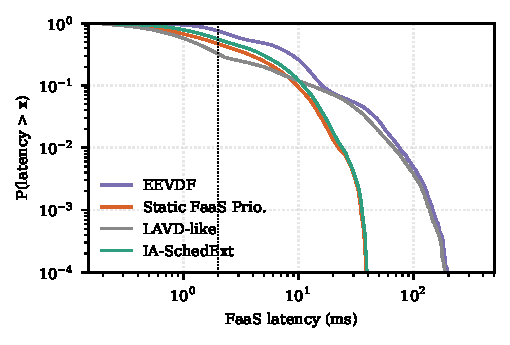
\includegraphics[width=0.95\columnwidth]{figs/fig_ccdf.pdf}
\caption{CCDF of FaaS latency on the bursty mixed workload (10 pooled runs). Dotted line: 2\,ms.}\label{fig:ccdf}
\end{figure}

\subsection{Single-class workloads}
\begin{table}[t]
\centering\scriptsize\setlength{\tabcolsep}{2.5pt}
\caption{Workloads A (FaaS only) and B (daemons only), 20 runs.}\label{tab:single}
\begin{tabular}{@{}llrrrr@{}}
\toprule
Workload & Scheduler & p50 & p99 & SLO (\%) & BG thpt\\\midrule
\SINGLETAB
\bottomrule
\end{tabular}
\end{table}
Without co-location (Table~\ref{tab:single}), IA-SchedExt matches EEVDF (p99 8.90 vs.\ 8.91\,ms), so the policy does not hurt pure-FaaS hosts, and all schedulers deliver 3.84 cores to daemon-only load.

\subsection{Mode behaviour, overhead, and sweeps}
On the bursty workload IA-SchedExt spends 31\% of time in FAIR, 19\% in STRICT, and 50\% in AGING (smooth: 24\%, 7\%, 69\%), and changes mode about 398 times per second (smooth: 470). Its modelled overhead is 0.03\% of CPU time; this follows from the assumed per-event costs and is not a hardware measurement. Figure~\ref{fig:sweeps} sweeps burst intensity and daemon count. Static priority is at or below IA-SchedExt's p99 everywhere, and the two converge when peak load exceeds capacity ($2.5\times$: 61.2 vs.\ 60.5\,ms), where every scheduler saturates. EEVDF and LAVD-like degrade steadily with more daemons (EEVDF p99 45.7\,ms with one daemon to 102.5\,ms with eight), while static priority stays flat (about 19.5\,ms) and IA-SchedExt rises from 19.9 to 27.1\,ms.

\begin{figure*}[t]
\centering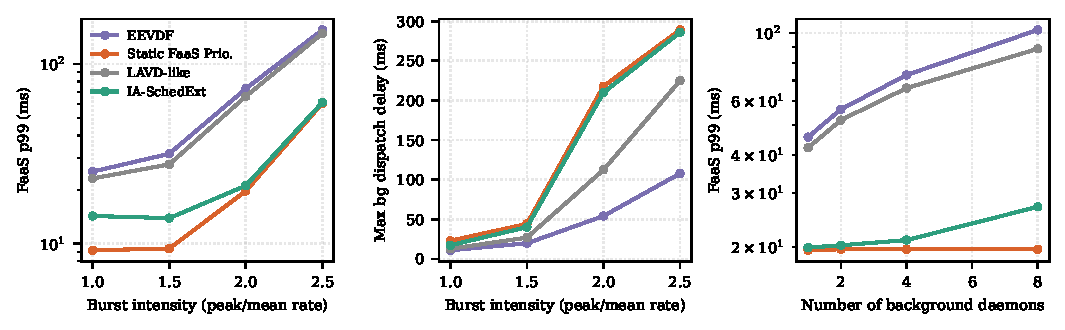
\includegraphics[width=0.95\textwidth]{figs/fig_sweeps.pdf}
\caption{Medians over 20 runs. Left/centre: burst intensity (mean rate fixed, $D{=}4$). Right: number of daemons (bursty, $2\times$).}\label{fig:sweeps}
\end{figure*}

\subsection{Ablations and sensitivity}
\begin{table}[t]
\centering\scriptsize\setlength{\tabcolsep}{2.5pt}
\caption{IA-SchedExt ablations and robustness, bursty workload, 30 runs (medians).}\label{tab:abl}
\begin{tabular}{@{}lrrrr@{}}
\toprule
Variant & p99 (ms) & SLO (\%) & BG max (ms) & Trans./s\\\midrule
\ABLTAB
\bottomrule
\end{tabular}
\end{table}
Table~\ref{tab:abl} shows that removing STRICT collapses p99 to 73.4\,ms (EEVDF-like), whereas removing AGING slightly \emph{improves} p99 (19.2 vs.\ 20.5\,ms) and SLO misses (29.2\% vs.\ 36.4\%): STRICT carries the whole benefit. Varying $\theta_{\mathrm{slo}}$ over 0.01--0.20 and the $F$ thresholds over 0.2/0.5--0.4/0.7 changes p99 by under 8\%, so the empirically calibrated thresholds are not fragile in this model. A 5 ms minimum dwell cuts transitions from 397 to 134 per second at unchanged p99, suggesting hysteresis is free. Classification error is the most damaging factor: 5\% misclassification raises p99 to 32.8\,ms (+60\%) and 20\% to 58.1\,ms. Finally, the interference strength $\gamma\in\{0,0.15,0.3,0.6\}$ moves EEVDF's p99 from 67.0 to 81.4\,ms but IA-SchedExt's only from 20.8 to 21.0\,ms.

\section{Discussion and Limitations}
\textbf{What the evidence supports.} Class-aware preemption of background work markedly reduces FaaS tail latency relative to EEVDF and a LAVD-like scheduler in the simulated mixed setting, and the gain is robust to threshold choice and to the strength of the assumed interference. It does \emph{not} support the claim that the three-mode machine beats strict FaaS priority: in the evaluated regimes strict priority is no worse for background work, because the daemons are elastic and FaaS demand stays below capacity on average. A benefit for the AGING mode would require regimes in which strict priority genuinely starves background tasks for long periods (sustained FaaS load near or above capacity, or background tasks with latency requirements); our $2.5\times$ burst case saturates all schedulers and does not show it.

\textbf{Limitations.} (1) All results come from a simulator whose EEVDF and LAVD models are approximations, and whose interference constants ($\gamma$, cache-refill and switching costs, telemetry costs) are assumed; no bare-metal PMC validation exists, and the reported 0.03\% overhead is modelled. (2) Classification is by an ideal oracle except in the misclassification sweep. (3) The AGING constants were tuned on a single workload family. (4) Workloads are synthetic, with 4 cores and no NUMA effects. (5) eBPF verifier limits may constrain richer heuristics. A sched\_ext implementation sketch is provided with the artifact but was not compiled or evaluated.

\textbf{Conclusion.} IA-SchedExt cuts simulated p99 FaaS latency by 71.5\% over EEVDF on a bursty mixed workload at no throughput cost, with its benefit coming entirely from strict-mode preemption; in this model a plain static FaaS-priority scheduler does as well or better, and the mode switching is noisy and sensitive to misclassification. Future work: real-kernel and trace-driven validation, workloads that stress background starvation, hysteresis and feedback-adaptive thresholds, and robust classification.

\section*{Data and Code Availability}
The simulator, tests, experiment scripts, raw results, and this paper's source are released in the accompanying archive; \texttt{run\_all.sh} regenerates every table and figure.

\begin{thebibliography}{9}
\bibitem{schedext} Linux Kernel Organization, ``sched\_ext: Extensible scheduler framework using eBPF,'' Linux v6.12 documentation, 2024--2026.
\bibitem{metis} W. Tang, Y. Yang, and J. Wu, ``Metis: A non-clairvoyant, workflow-aware OS scheduler for serverless applications,'' in \emph{Proc. ACM SoCC}, 2025, pp. 112--126.
\bibitem{emfs} Anonymous, ``eMFS: Interference-aware scheduling via eBPF and meta-learning,'' in \emph{Proc. PACMI}, 2025.
\bibitem{apsys} System Research Group, ``High-performance eBPF-based OS scheduling for serverless functions,'' in \emph{Proc. APSys}, 2026.
\bibitem{lavd} C. Chang, ``LAVD: A BPF scheduler for cloud, ML, and edge,'' in \emph{Linux Plumbers Conf.}, 2025.
\bibitem{platbal} FaaS Infrastructure Group, ``Serverless platform driven CPU load balancing,'' arXiv:2504.09123, 2025.
\bibitem{musched} Y. Zhang \emph{et al.}, ``MUSched: Interaction-aware CPU scheduling for mobile,'' in \emph{Proc. USENIX OSDI}, 2026.
\end{thebibliography}
\end{document}
